\documentclass[a4paper,chapter,11pt]{oblivoir}

%%%%%%%%%%%%%%%%
% Front Matter %
%%%%%%%%%%%%%%%%

\usepackage[utf8]{inputenc}       		% For setting encoding
\usepackage[margin=1in]{geometry}		% For setting page margins
\usepackage{booktabs}             		% For table rules
\usepackage{setup/ob-chapstyles}
\usepackage{graphicx}             		% For adding figures
\usepackage{float}                		% For floating environment
\usepackage{longtable}            		% For long tables
\usepackage{caption}              		% For custom captions
\usepackage{subcaption}
% \usepackage[acronym,toc]{glossaries}	% For making glossaries
% \usepackage[doublespacing]{setspace}	% For setting line spacing
% \usepackage{times}						% For using times font
% \usepackage{kotex}		    			% For using Korean text
\usepackage{setup/kotex-sections}		% For using Chapter, Section Name in Korean
\usepackage{lipsum}						% For using random text
% \usepackage{todonotes}					% For adding to-do notes
\usepackage{hyperref}					% For cross-referencing
\usepackage[backend=bibtex8,style=ieee]{biblatex}
\usepackage{mwe}                        % loads »blindtext« and »graphicx«
\usepackage{scalerel,amssymb}
\usepackage{listings}
\usepackage{enumitem}
\usepackage{minted}
\usepackage[english]{babel}
\usepackage{amsmath}
\usepackage{tikz}
\usetikzlibrary{arrows,automata}

\addbibresource{ref.bib}
\def\msquare{\mathord{\scalerel*{\Box}{gX}}}
\usepackage{epstopdf}
\epstopdfDeclareGraphicsRule{.tif}{png}{.png}{convert #1 \OutputFile}
\AppendGraphicsExtensions{.tif}

\renewcommand\thesubfigure{(\alph{subfigure})}
\captionsetup[sub]{
  labelformat=simple
}
\def\figureautorefname{그림~}


% \kscntformat{section}{제~}{~장}								% Declare packages

%%%%%%%%%%
% Title, Authors, Date %
%%%%%%%%%%
\title{오버워치 가이드}

\author{순수이성비판\#31307}
\date{\today}

\begin{document}

% \title{마이크로프로세서실험 Lab1 보고서}
% \author{20181485 고재현}
% \date{10 May 2021}
%%%%%%%%%%
% covers %
%%%%%%%%%%

% \input{covers/cover_outer.tex}					% Text for outer cover
% \input{covers/cover_inner.tex}					% Text for inner cover
% \input{covers/judges.tex}				    	% Text for inner cover


%%%%%%%%%%%%%%%%%%%%%
% Table of Contents %
%%%%%%%%%%%%%%%%%%%%%
\maketitle

\begin{abstract}
이 문서는 오버워치를 플레이하는 사람들이 참고할 만한 상황별 가이드를 제공하는 것을 목적으로 작성되었다.\\
승리를 목적으로 의도적으로 구성된 영웅 모음을 조합이라고 한다면 오버위치 최상위 경쟁전과 프로경기는 해당 패치에서 최강인 조합 즉 메타 조합을 찾는 과정인 '과도기' 를 지난 뒤, 각 팀의 메타 조합의 운영 숙련도를 겨루는 '안정기' 두 phase로 구성되어 있었다.\\
이에 오버워치 개발진은 메타 조합을 없애기 위해 패치를 거듭하고 있다. 단적인 예로 이 서문이 작성되고 있는 21년 7월에는 로드호그의 고철총 데미지의 미세한 조정을 통해 OP와 쓰레기 사이의 어느 지점에 수렴하도록 노력 중이다. 현 시점, 리그나 최상위 경쟁전의 영웅 사용 빈도를 살펴보면 특정 영웅을 특정 전장에 사용하거나 팀 컬러에 맞는 영웅을 사용하고 있는 것을 확인할 수 있다. 즉 메타 조합을 따로 찾지 않아도, 각 영웅들의 시너지를 만들 수 있도록 조합을 구성하고 알맞게 운영한다면 승리라는 목적을 쟁취할 수 있다.\\
이를 뒤집어서 생각하면 이제는 어느 영웅을 기용할지 면밀하게 생각함과 동시에 상황에 따라 다르게 운영해야 한다. 이에 대한 판단 기준을 1편에서 마련하고 기준에 따른 판단 결과, 즉 각 영웅의 상황별 운영법과 피지컬 훈련법을 2편에서 살펴본다.
\end{abstract}

\pagenumbering{roman}                           % Start page numbering in Roman numerals
\tableofcontents*        						% Add table of contents
%\thispagestyle{empty}							% Suppress the page number
\clearpage
\oblivoirchapterstyle{obbianchi}

%%%%%%%%%%%%%%%%%
% preliminaries %
%%%%%%%%%%%%%%%%%

% \addcontentsline{toc}{section}{\listfigurename} % Add list of figures to table of contents
% \listoffigures									% add list of figures
% \clearpage

% \addcontentsline{toc}{section}{\listtablename} 	% Add list of figures to table of contents
% \listoftables									% Add list of figures
% \clearpage

% \input{text/abstract_korean}		      		% Text for Korean Abstract

\setcounter{table}{0}		                    % Reset table counter
\setcounter{figure}{0}		                    % Reset figure counter

%%%%%%%%%%%%%
% Main Text %
%%%%%%%%%%%%%

\pagenumbering{arabic}							% Start page numbering in Arabic numerals

% \chapter{목적}{\label{sec:purp}}
다음의 세 가지 이해를 바탕으로 관찰, 계획, 실행, 피드백의 의식적 네 단계가 무의식을 지배하는 것을 목적으로 한다.\footnote{polya의 문제 해결 4단계를 차용한 것이다.}
\begin{enumerate}
    \item 연습에 대한 체계적인 이해
    \item 피지컬에 대한 체계적인 이해
    \item 뇌지컬에 대한 체계적인 이해
\end{enumerate}
	
% \clearpage


					    % chapter 1
% \part{피지컬}
\chapter{에임}{\label{chap:aim}}
\section{introduction : 에임의 목표와 요소}
에임의 목적은 시선과 크로스헤어, 즉 마우스 움직임의 동기화이다. 즉, 내가 보는 곳으로 에임을 옮기는 것이다. 따라서 에임을 하기 위해서는 우선 눈으로 상대를 인식해야 하며, 마우스를 옮겨 크로스헤어를 상대 위에 가져다두어야 한다. 그리고 마우스를 옮기는 동작은 팔에 달린 수많은 근육과 힘줄이 수행한다. 여기까지의 논의를 바탕으로 에임 연습의 목적은
\begin{enumerate}
    \item 팔과 손목, 손가락의 움직임과 마우스의 움직임 사이의 관계를 익히고
    \item 마우스의 움직임과 크로스헤어의 움직임 사이의 관계를 익혀서
    \item 신체의 움직임과 크로스헤어의 움직임을 연결하는
\end{enumerate}것이라고 할 수 있다.\footnote{마우스의 움직임과 크로스헤어의 움직임 사이에는 1대1대응 및 선형성이 성립하지만, 근육의 움직임과 마우스의 움직임 사이에는 선형성은 보장할 수 없으므로 학습이 필요하다.}
그러므로
에이밍은 시선, 자세, 감도, 관절가동범위, 지지대 등 수많은 요소들이 복합적으로 작용하는 동작이라고 할 수 있다. 에임을 쉽게 맞추기 위한 뇌지컬적, 피지컬적 요소들을 정리해 보고, 에임을 볼안정하게 만드는 요소는 무엇인지, 어떻게 연습해야 안정적이고 부상 없는 에임을 유지할 수 있는지 등을 알아보자.


\section{자세}
에임을 옮기려면 마우스(정확히는 중앙에 있는 센서 부분\footnote{tip을 하나 주자면, 마우스 센서를 연필심이라고 생각하고 글자를 쓴다고 생각해 보자.})를 옮기거나 키보드를 눌러 조정해야 한다. 그런데 키보드를 누르고 마우스를 옮기는 신체부위는 전완을 포함한 굉장히 많은 근육들 및 손가락을 움직이기 위한 힘줄들이다. 이때 이 근육들을 오래동안 아프지 않게 사용하려면 바른 자세로 게임해야 한다. 게임을 하다보면 습관적으로 체중을 발바닥, 좌골뼈(엉덩이), 등과 허리가 아닌 책상의 경계면과 팔이 맞닿는 부분 또는 손목 등 말단부위에 체중을 싣게 되는데, 이 경우 신경이 눌리면서 통증을 유발하고, 마우스에 과도한 힘이 들어가면서 에임을 불안정하게 만들기 때문이다.
바른 앉기 자세에 대해서는 의학적으로 여러 논문이 나와있다. 피지컬갤러리의 앉기에 관한 영상\cite{pg_sitting}을 찾아보면, 두 발은 바닥에 제대로 닿아있고\footnote{https://youtu.be/TmiSDn0nF90}, 좌골뼈가 의자의 바닥에 닿으면서, 등은 전체적으로 등받이에 기대고, 정강이와 팔꿈치 윗부분은 상체와 평행한 상태가 신체에 부담을 주지 앉는 자세라고 한다. 이를 자세하게 알아보자.
    \begin{figure}[h]
         \centering
         \begin{subfigure}[b]{0.3\textwidth}
             \centering
             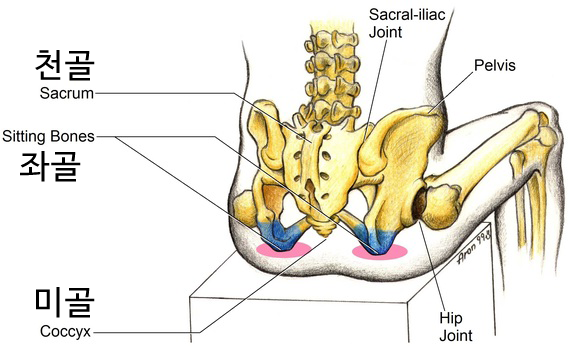
\includegraphics[width=\textwidth]{figures/sit.png}
             \caption{앉을 때의 좌골뼈의 위치}
             \label{fig:sit}
         \end{subfigure}
         \hfill
         \begin{subfigure}[b]{0.3\textwidth}
             \centering
             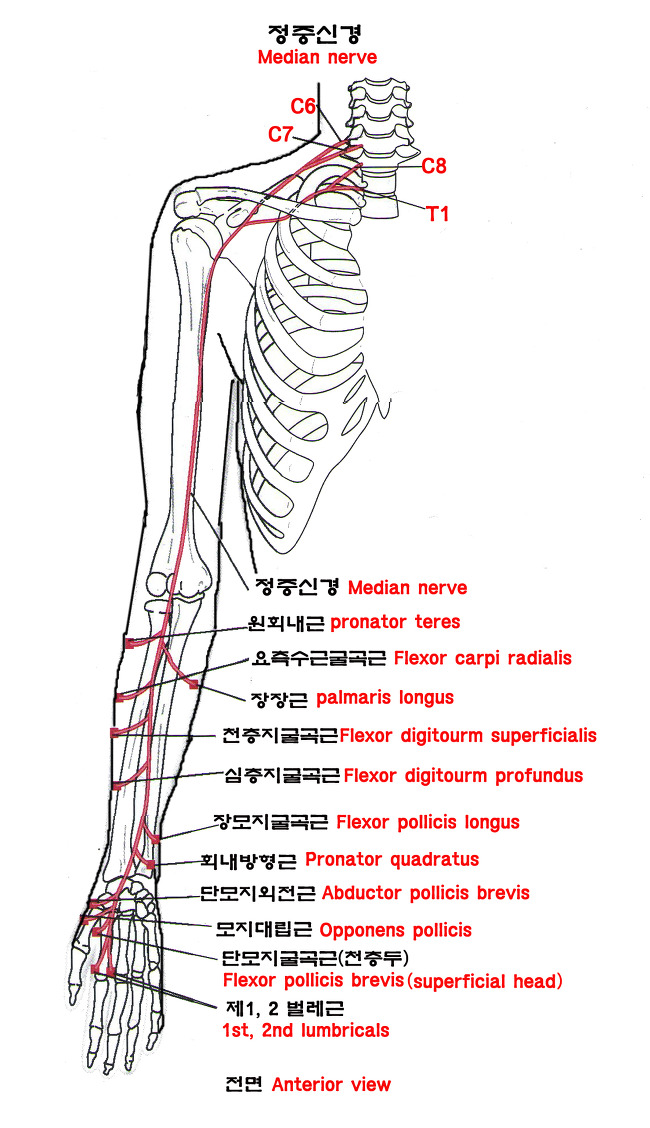
\includegraphics[width=\textwidth]{figures/med_nerve.jpg}
             \caption{정중신경이 지나는 모식도}
             \label{fig:1-b}
         \end{subfigure}
         \hfill
         \begin{subfigure}[b]{0.3\textwidth}
             \centering
             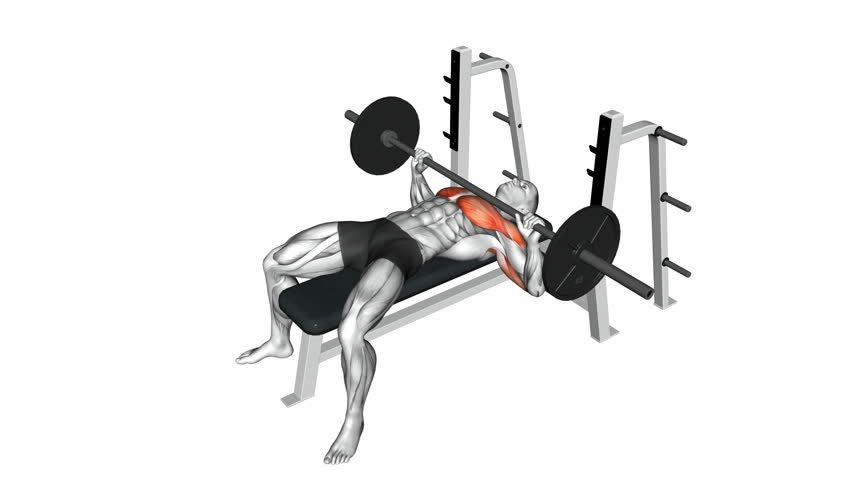
\includegraphics[width=\textwidth]{figures/bench.jpg}
             \caption{벤치프레스 자세}
             \label{fig:1-c}
         \end{subfigure}
            \caption{자세에 관한 이미지 자료}
            \label{fig:impl1}
    \end{figure}

몸의 맨 위쪽부터 알아보자. 눈높이는 모니터의 맨 위쪽 선에 맞추자. 턱은 당기고, 목은 펴주고, 어깨가 들리지 않게 의자의 높이 또는 책상의 높이를 조절해야 한다. 이 때, 어께의 좌우벨런스가 틀어지지 않도록(측만증) 주의하자. 가슴은 펴고, 등은 의자 등받이에 전체적으로 닿게 기대주자. 정중신경의 모식도를 보면 알겠지만, 어께가 앞으로 굽게 되면 해당 신경이 눌리면서 터널증후군을 유발하므로 유의하자. 팔은 팔꿈치 위쪽은 상체와 평행하게 두되 몸통과 팔 사이의 각도를 크게 해서 팔 에이밍시 어께가 돌지 않도록 한다. 팔꿈치를 몸통에 붙이고 팔에임하면 어께가 돌아가는 게 느껴짐. \footnote{꼭 완전히 평행할 필요는 없다! 그러나 팔이 너무 앞으로 나가서-이 경우 어께-팔꿈치 부분과 몸통과의 각도가 30도 이상으로 커지면 신경 눌려 통증 생김 라운드숄더가 되거나 힘줄이 당겨지지 않도록 주의하자.}, 팔꿈치 아래는 마우스패드와 수직하게 마우스패드에 살짝 올려준다. 이 때 회전축이 되는 손목과 팔꿈치의 특정 위치에 무게를 싣게 되면 통증을 유발하니, 패드에 살짝 대준다는 느낌으로 축을 설정해야 한다. 게다가 축을 세게 누르면 에임범위를 벗어나는 대상에 에이밍하거나 상하에임 시 축이 드드득거리면서 부드러운 에이밍이 불가능해진다. 이를 요약하면, 마우스를 들고 움직이는 게 아니라 친다고 생각하면 좋다.
허벅지는 의자에 닿도록, 양 발은 바닥을 지지해야 한다. 이때 발이 바닥에 닿지 않으면 발받침대를 구해서 사용하자. 발이 제대로 지지가 안 되면 무게중심이 앞으로 가면서 팔과 손목에 체중이 가해지니 주의해야 한다. 즉 몸 전체의 무게중심을 고르게 해야 패드 위에 올라간 부위의 무게중심도 고르게 분포된다. 등받이에 등이 전체적으로 닿는 것도 같은 맥락에서 중요하다. \footnote{어릴 때 의자에 엉덩이 끝까지 붙이고 앉으라고 했던 말이 사실 팔도 아프고 손목도 시큰거리게 되니까 했던 게 아닐까?} 이상으로 정리한 자세는 상체의 모양은 벤치프레스 자세와 유사하고, 어깨 아래 부분은 손걸레질 하는 자세랑 유사하다. 
이제 바르게 앉은 상태에서 팔을 편안하게 책상 위에 올려놓자. 어께와 팔의 모든 부분에 긴장이 풀리도록 해보자. 그게 당신의 에이밍 자세이다.

\section{근육과 축}
손을 움직이려면 전완근의 수축과 이완이 필요하고, 팔을 움직이려면 대흉근과 삼각근의 수축과 이완이 필요하다. from bardoz


\section{사운드플레이, crosshair replacement, peek}
에임의 상황을 화면과 조준선(화면의 중앙) 기준으로 에임의 상황을 나누어 보자. 상대가 내 화면(순간 에임범위 이내) 안에 있는지 여부와 조준선 위에 있는지 여부라는 기준으로 3가지 상황으로 나누어진다. 상대가 내 화면 밖에 있는 경우에는 상대가 발사하는 총알의 궤적, 사운드 등을 이용해 상대의 위치와 동선을 예측해서 헤드라인 근처에 에임을 대고 나가야 한다. 이를 peek이라고 부른다.
상대가  내 화면 안에 있는 경우, 상대를 조준선 위에 얹고 따라가면 된다. 상대가 내 크로스헤어 위에 있는 경우, 트레킹만 하면 된다.
에임범위 밖의 대상을 에이밍한 뒤에는 마우스를 들어서 팔과 손목을 다시 편한 위치로 옮겨주자. 이를 crossehair replacement라고 한다.

\section{키보드 에이밍}
오버워치는 움직임에 따른 반동이 없는 게임이기 때문에 키보드의 움직임을 에임에 활용할 수 있다.  캐릭터간 이동속도는 거의 동일하므로, 서로 좌우무빙을 치면서 교전중일 때, 나는 상대 몸 위에 크로스헤어를 올려둔 상태라면 상대가 나와 같은 방향으로 움직이면 에임을 위아래로만 움직이면서 쏘면 다 맞출 수 있다. 좌우 방향으로 상대속도가 0이기 때문이다. 상대가 나와 반대 방향으로 움직이면, 내가 가만히 서서 쏠 때보다 2배 빠른 속도로 마우스를 움직여야 한다. 이 경우 내 에임범위를 금새 벗어나게 되므로, 축을 풀어주지 않으면 트레킹이 끊기게 된다. 무빙을 적당히 섞을 경우 에임범위 문제를 어느 정도 해결할 수 있다. 
\subsection{위도우의 점프샷}
\footnote{https://youtu.be/T-sucESdZPQ}
\begin{enumerate}
    \item 상대가 있을 위치에 에임 미리 대기
    \item 줌부터 누르고 점프 후 방향키(차징을 위함)
    \item 벽이 좁으면 제자리에서 점프 후 줌 누르고 방향키
    \item 최종 위치는 상대의 위치와 벽 경계선을 일자로 둔다.
\end{enumerate}
\subsection{위도우의 훅샷}

\section{정보처리}
\subsection{상대가 주요시야범위 밖에 있을 경우}
사운드, 총알궤적으로 상대 케릭터의 헤드라인을 미리 잡아둔다.
\subsection{상대가 주요시야범위 안에 있을 경우}
\subsubsection{상대의 움직임 경로와 내 움직임 경로는 어떻게 하지}
\subsubsection{상대가 내 크로스헤어 밖에 있을 경우}
\begin{enumerate}
    \item 상대의 이동방향과 내 크로스헤어의 이동방향이 같은 경우
    \item 상대의 이동방향과 내 크로스헤어의 이동방향이 반대인 경우
\end{enumerate}
\subsubsection{상대가 내 크로스헤어 안에 있을 경우}
에이밍할 때는 목표지점과 목표가 움직이는 방향을 봐야 한다. 크로스헤어는 주변시아로 확인하며 크로스헤어를 상대 위에 올려놓기 위해 목표지점과 화면 중앙 사이의 거리를 계산하는 용도로 사용한다.
상대의 무빙을 예측하는 건 사람의 반응속도 한계 때문에 큰 도움이 안 된다. 예측은 상대의 동선을 생각하는 데에 사용하고, 캐릭터가 움직이는 방향에 따라 모양이 달라지는 점을 이용해서 무빙을 보고 쏘도록 하자. 예를 들어 루시우의 경우
    \begin{figure}[htp]
         \centering
         \begin{subfigure}[b]{0.3\textwidth}
             \centering
             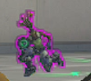
\includegraphics[width=\textwidth]{figures/read_moving/left.png}
             \caption{왼쪽으로 움직이는 경우}
             \label{fig:1-a}
         \end{subfigure}
         \hfill
         \begin{subfigure}[b]{0.3\textwidth}
             \centering
             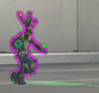
\includegraphics[width=\textwidth]{figures/read_moving/l2r.png}
             \caption{왼$\rightarrow$오의 뱡향전환}
             \label{fig:1-b}
         \end{subfigure}
         \hfill
         \begin{subfigure}[b]{0.3\textwidth}
             \centering
             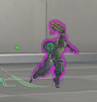
\includegraphics[width=\textwidth]{figures/read_moving/right.png}
             \caption{오른쪽으로 움직이는 경우}
             \label{fig:1-c}
         \end{subfigure}
            \caption{루시우의 움직임}
            \label{fig:read_moving}
    \end{figure}
와 같이 움직임에 따라 모양이 달라지고, 이는 에이밍에 활용할 만한 정보이다. //
연습 방법은 다음과 같다.
\begin{enumerate}
    \item ctrl+z를 눌러 UI를 끈다.
    \item 이 상태에서 상대의 움직임을 파악한 뒤 마우스로 이를 따라간다.
    \item 움직임 관찰 단계의 문제인지, 운동수행능력의 문제인지 파악한다.-방향전환은 속도가 느려지므로 더 디테일한 축을 활용해야함
    \item 문제를 해결한 뒤 2번으로 돌아간다.
\end{enumerate}
%FPS에서의 에임은 구면좌표계 위를 움직이게 된다. 하지만 내가 보고 있는 화면은 평면이므로, 그냥 상대를 바탕화면에 놓인 아이콘이라고 생각하고 클릭하자고 생각하면 도움이 될...수도 있다.

\section{상대의 움직임 경로, 범위}
상대의 주의력 자원에 대해서 생각해보자. 상대가 나를 의식하지 못할 때 쏘는 게 좋다.\footnote{볼트 포커싱이 강력한 이유} 무빙치는 적은 상대하기 까다롭다. 상대의 움직임 경로와 범위를 생각하면서 에임하면 쉽다. 예를 들어 리스폰에서 갓 나온 적은 직선으로 움직인다거나, 겐지의 이단점프는 높이 최대값이 어느정도 정해져있다는 점 등이다.


\section{감도}
감도는 자주 바꾸지 말고 하나 정해서 움직임을 훈련한다. 오버워치의 경우, 상대가 매우 빠르게 움직이므로 좌우로 180도는 커버할 수 있는 감도가 좋고, 이 감도는 보통 edpi 4000 언저리의 중감도이다.\footnote{필자는 800dpi 4.5, zoom-sens 30}

\section{힘조절}
일단 에임의 기초가 없는 사람들은 힘을 쭉 풀어주고 연습하자. 에이밍할 때 작용하는 힘은 마우스를 마우스패드에 수직한 방향으로 누르는 힘과 마우스를 미는 힘 두 가지가 있다. 상대가 크로스헤어를 기준으로 멀리 있거나, 빠르게 움직인다면 누르는 힘을 줄이고 미는 힘을 늘려야 하고, 가까이 있거나 느리게 움직이면 누르는 힘을 키우고 미는 힘을 늘려야 한다. 이 때 누르는 힘을 가했다가 다시 풀어주는 것이 중요한데, 자세가 잘못되어 무게중심이 엉덩이가 아니라 손과 팔로 옮겨지게 되면 누르는 힘을 다시 풀기 어려워져 에임이 점점 안 맞기 시작하니 주의하자. 마우스를 미는 힘은 다시 상하로 미는 힘과 좌우로 미는 힘으로 구분할 수 있는데, 상하에임의 경우 어께를 축으로 팔 전체를 위아래로 옮기거나 손가락으로 마우스를 위아래로 옮기는 방법이 있고, 좌우로 미는 힘의 경우 팔을 축으로 미는 힘과 손목을 축으로 미는 힘, 마우스를 축으로 손가락으로 미는 힘 세 가지가 있다. 이제 이 미는 힘과 누르는 힘을 연습해보자. AIMLAB은 STEAM에서 무료다!

\section{축}
안정감 있게 에임해야 할 때는 신체부위 한 곳을 지지대삼아서 트래킹하거나 끌어치기하면 안정감이 더해진다. 예를 들어 손목을 대고 손인사하듯 좌우로 까딱거리면 헤드라인 끌어치기가 쉽다. 이렇게 에이밍의 안정성을 위해 축을 설정하고 풀 수 있어야 한다. 이 때 주의할 점이 몇 가지 있다. 팔에임과 손목에임을 구분하여 팔 끝까지 쓴 후 손목을 움직이는 게 아니라 모든 관절을 섞어쓸 수 있어야 에임이 부드러워진다. 축을 설정할 때 팔꿈치부터 손목까지의 무게중심은 고르게 설정되어야 한다. 그렇지 않으면 상하에임 도중 손목이 들리면서 충격을 줄 수 있기 때문이다. 셋째로, 손목과 팔이 편하게 가동되는 범위까지만 움직여야 하고 그 이상은 사용하지 않아야 한다.

\section{마우스 그립}
마우스 그립법은 마우스 위에 손을 올려놓는 방법을 의미한다. 이 방법에는 여러 가지가 있으며 마우스의 모양과 유저의 신체조건에 따라 달라진다.
마우스 그립에 따라서 손목의 가동범위, 힘줄 및 신경에 주는 압력, 팔의 외회전 정도 등의 많은 요소가 달라진다. 가장 유명한 그립법은 팜, 클로, 핑거팁의 세 가지 그립법이지만 131 그립과 같이 손목을 중립에 두어서 가동범위의 대칭성을 맞춰주는 방법 등 다양한 그립법이 존재한다. 마우스 쉘의 모양과 무게 분포 및 유저 개개인의 손 크기 등 신체조건에 따라 마우스 그립을 다르게 해야 손목건강과 안정적인 에임을 유지할 수 있다.
- figure 추가할 것
마우스 양옆을 강하게, 윗면은 힘 빼야함 연필 잡는 것과 동일하게 생각, 단 중지와 검지가 컨트롤에 활용됨


\section{에임범위}
마우스를 옮기는 직접적인 신체부위는 팔꿈치와 손목, 손가락이다. 손끝에 가까운 부위를 사용할수록 한 번에 옮길 수 있는 범위가 좁아지지만 정밀한 마우스 컨트롤이 가능하고, 손끝에서 먼 부위를 사용할 수록 한 번에 옮길 수 있는 범위가 커지지만 정밀한 마우스 컨트롤이 어렵다. 또한, 일반적으로 신체구조상 왼쪽으로의 에임범위가 오른쪽으로의 에임범위보다 좁으므로 연습할 때 이를 고려해야 한다. 에이밍을 연습하기 전에, 바르게 앉은 상태에서 본인의 관절에 무리를 주지 않는 선에서의 각 부위별 에임 범위를 파악하고 있어야 한다.\\
 팔꿈치쪽 축으로부터 마우스 센서까지의 거리를 l,  손목쪽 축으로부터 마우스 센서까지의 거리를 r이라고 하자. l이 시작상태에서 움직인 각도를 $\theta$, r이 시작상태에서 움직인 각도를 $\alpha$ 라고 하면(당연히 단위는 radian), 마우스가 호를 따라 총 움직인 거리는 $l\theta+r\alpha$ 로 구할 수 있다. 이 때 마우스를 좌우로 움직이려면 직선으로 움직여야 하는데 각도가 너무 크면 직선이 아니라 곡선으로 움직이게 됨을 유의하자. 이를 막기 위해서는 축을 기준으로 팔과 손목을 까딱거린다고 생각하기보다는 마우스의 움직임에 집중하면 좋다.




\section{셀프 피드백 : 문제 판단 후 해결}
어느 정도 기초가 잡혔다면, 에이밍을 하면서 왜 안 맞는지 고민해서 수정할 수 있어야 한다. 대표적인 경우로 상대 몸 위에 크로스헤어를 올려놓지 못했는데 상대의 동선을 마우스로 따라가고 있는 상황이 있다. 이 경우에 상대의 위치가 내 에임범위 이내라면 끌어치기를 살짝 섞어서 크로스헤어를 올려놓고 트레킹하면 되고, 상대의 위치가 내 팔꿈치의 가동범위 밖이라면 팔꿈치 근처의 축을 풀고 팔을 전체적으로 이동시켜서 에이밍하거나, crosshair replacement 한 뒤 에이밍하면 된다. 이처럼 본인이 왜 안 맞는지 생각해보고 의식적으로 수정한 에이밍 방법이 무의식적으로 굳어진 습관을 이길 때까지 연습해보자. 연습은 마우스를 습관대로 까딱까딱거리는게 아니라 더 좋은 방법을 생각하고 무의식적으로 굳어진 습관을 의식적으로 덮어씌우는 과정이라는 걸 잊지 말자. 그리고 이론에 너무 매몰되지는 말자. 이 장의 목적은 건강하게, 잘, 게임하는 것이다!
% \part{뇌지컬}
 \chapter{오버워치의 자원}{\label{sec:res}}
% 뭘 쓰는게 좋을까요?
\section{introduction : 오버워치의 자원?}\label{res:intro}
오버워치는 서로의 자원을 교환하며 상대의 진입은 막고, 아군의 진입은 돕는 게임이다. 오버워치에서의 자원의 종류와 특징에 대해서 알아보고, 어떻게 자원을 교환해야 유리한 게임이 진행되는지 생각해 본다.

오버워치의 자원
자원의 획득
자원의 소모 -교환
자원의 낭비
자원의 흡수
자원의 상대성
자원의 순환


%  레킹볼을 플레이할 때 아군의 주는 방벽을 받고 굴러다니면서 수면총과 방패 밀쳐내기 등 CC기를 빼면서 보호막을 채우고, CC기 사이클이 돌기 전에 파일드라이버를 사용하면 상대는 '주는 방벽' 이라는 낮은 코스트 기술에 CC기를 소모하였으므로 파일드라이버 후 CC기 포커싱을 사용할 수 없게 된다. 레킹볼 입장에서는 상대의 견제가 약해졌으므로 오랜 시간 동안 어그로를 끌 수 있다.
% 마지막으로 상대방 용검턴에 지원가가 빠져있는다거나, 자탄턴에 팀원이 나누어 자리를 잡으면 템포를 늦출 수 있다.

\section{자원의 종류}
\subsection{주의력}
신경론
시야, 사운드
\subsection{체력}
오버워치의 체력에는 네 가지 종류가 있다.
\begin{enumerate}
    \item 아머 : 한 대당 데미지 3씩 감소시켜주는 체력이다. 탱커들의 아머를 채워주면 최대한의 힐 효율을 볼 수 있다.
    \item 파란색 보호막 : 상대의 궁극기를 채워주지 않는다.
    \item 하늘색 보호막 : 데미지를 입지 않고 3초 이상 있으면 다시 채워지는 체력이다.
    \item 흰색 체력 : 가장 일반적인 체력이다.
    
\end{enumerate}
\subsection{기본공격, 스킬, 궁극기}
각 영웅의 기본공격과 스킬, 궁극기라는 자원은 다음 여섯 가지 목적으로 구분할 수 있다.
\begin{enumerate}
    \item 이동
    \item 이동 방해
    \item 힐
    \item 힐 차단
    \item 딜링
    \item 딜 차단
\end{enumerate}
\subsection{지형 calling}
코너 기준 번호판처럼 생각, 위 아래로 구분
\subsection{지형과 포지셔닝}
\begin{enumerate}
    \item 고지대는 왜 중요할까?
     오버워치를 하다 보면, 마스터 후반 유저들부터 고지대싸움을 치열하게 하는 모습을 볼 수 있다.
     그 이유는 고지대를 뺏으려고 진입하던 중에 변수가 생기거나, 자원이 소모되거나, 
\end{enumerate}

    % \begin{figure}
    %     \centering
    %     \includegraphics[scale = 0.2]{figures/step5.png}
    %     \caption{STEP 1 ~ STEP 5를 수행한 후 μvision 화면}
    %     \label{fig:step5}
    % \end{figure}
 
% \clearpage

\chapter{자원의 평가 요소}
자원을 사용하게 되면 상대가 반응하여 자원을 소모하게 된다. 또는 상대가 자원을 사용했을 때 반응하여 자원을 사용하게 된다. 이 때 자원 사용의 결과를 예측하고 가장 좋은 결과를 낼 수 있는 방식으로 자원을 투자하려면 평가의 기준이 필요하다. 자원 사용의 결과를 평가하는 기준으로 시간과 공간, 그리고 상대의 자원이라는 세 가지 관점을 알아보자.
\section{시간 : 오버워치의 흐름이자 플레이의 기준}
오버워치에는 탄창, 체력, 스킬 등의 여러 자원이 존재하고, 이 자원들의 공통점은 사용하고 나면 다시 채워야 한다는 점이다. 채우는 데에는 시간이 필요하고, 이 시간동안 캐릭터는 약해지거나 무력해진다. 예를 들어, 구르기가 없는 맥크리는 장전에 1.2초가 걸리고, 메르시의 부활 캐스팅 시간은 1.75초이므로 탄창을 세서 부활타이밍을 잴 수 있다.
파라의 부스터 재사용 대기 시간은 8초이며 메르시가 이 시간을 생각하며 이동하면 파라를 시선에서 놓치더라도 쉽게 발견할 수 있다. 이처럼 오버워치에는 사이클이 존재하며 이 사이클마다 정보수집(Read),상황판단(Decision making),계획(Plan),실행(Do),피드백(Feedback)의 다섯 단계를 밟아나가야 한다.
오버워치의 시간 사이클은 세 가지로 구분할 수 있다.
\begin{enumerate}
    \item 10초 내외의 각 캐릭터의 사이클\label{cyc:1}\\
    이 사이클은 스킬을 사용하고 쿨타임 동안, 체력이 빠지고 다시 채울 때까지의 사이클이다. 섬광탄이 빠진 맥크리는 레킹볼-트레이서 포커싱에서 살 수 없다. 체력이 빠진 젠야타는 다시 채워지기 전까지 자리를 옮기기 어렵다. 이러한 각 영웅의 사이클이 한타의 사이클을 만드는데, 각 팀 탱커의 스킬을 기준으로
    \begin{itemize}
        \item 아군의 진입턴 : 어떻게 킬을 낼 것인가? 상대가 버티는 것을 어떻게 차단할것인가?
        \item 상대의 진입턴 : 어떻게 버틸 것인가? 잘 하면 역으로 변수를 만들 수도 있지 않을까?
    \end{itemize}
        
    이 결정된다. 라자조합에서의 자리야 방벽 및 라인하르트 방벽, 윈디조합에서의 호빵 및 매트릭스가 이에 해당한다. 여기에 나머지 영웅의 궁극기 등 자원상황을 추가적으로 고려한다. \textbf{이는 오버워치 플레이의 가장 중요한 기준이 된다.}두 턴 모두에서 주의해야 할 점은 내가 죽지 않는 것, 아군을 죽이지 않으면서 상대를 죽이는 것이다. 이 관점을 기준으로 각 포지션의 역할을 생각해보자. 아군의 진입턴에서의 각 포지션별 역할을 가볍게 생각해보자. 아군의 진입턴에서 탱커는 
    아군의 힐각과 딜각 생각하면서 진입하기. 진입의 근거 만들기. 예) 상대 방벽이 없고 우리는 있을 때, 상대 힐벤이 빠졌을 때 진입한다.
    \item 30초에서 1분 내외의 한타 준비-전개 단위 사이클\\
    이 사이클은 \nameref{cyc:1}이 여러 번 반복되는 네 단계로 이루어진다. 이 때 단계는 \nameref{cyc:1} 의 1회 수행마다 한 단계가 진행될 수도 있고, 여러 단계가 진행될 수도 있고, 궁극기 파밍 외에 아무런 소득도 없을 수도 있다.
    \begin{enumerate}
        \item pre-fighting: 대치와 한타 계획 \\
        한타 이전에는 이 다음에 벌어질 한타를 위해 자원을 모으고 한타 과정을 계획해야 한다. 특히 첫 싸움의 경우 한타 계획 단계에서 서로의 조합을 비교해야 한다.
        \begin{itemize}
            \item 조합 변경점 체크하기. 마지막 턴이고 아군이 가진 수비궁이 없지만, 상대가 중력자탄을 가지고 있다면 지원가가 바티스트, 탱커가 디바를 꺼내서 카운터를 시도할 수 있다. 상대가 조합 변경점을 인지하지 못한다면, 매트릭스에 차단당할 확률이 높을 것이다. 이와 같이, 조합의 변경점을 체크한 상태에서 플레이를 준비해야 한다.
            \item 상대가 가진 자원과 아군이 가진 자원 계산하기: 주로 궁극기를 체크하고 상대의 궁극기를 카운터할 방법과 아군의 궁극기 사용 및 효율적인 포커싱, 힐을 위한 동선과 스킬 사용 순서를 계획한다. 초심자는 "오버워치는 턴제 궁극기 교환 싸움이다."  "궁극기는 2턴마다 한번씩 돈다" "궁극기를 카운터할 수 있는 방법은 여러 가지이다" 만 우선 기억하도록 하자.
            \item궁극기 계산 요소
            \begin{enumerate}
                \item 상대의 딜량 기반으로 예측하기 예) 화염강타 한대당 10\%
                \item 아군의 힐량 기반으로 예측하기 예) 아군 힐러 궁이 빠르면 상대 딜러들의 궁이 빠름
                \item 아군의 플레이방식, 적군의 플레이방식 기반으로 예측하기 예) 겐지가 뒷라인 암살만 노릴 때보다 앞라인과 딜교환을 오래하면 용검이 20초정도 빨리찬다. 
            \end{enumerate}
            \item 아군이 가진 자원을 적절히 사용하기 위해 상대가 가진 자원을 소모시키기. ex)화강, 모이라 구슬으로 매트릭스 빼고 자탄, 자탄 쓰기 전에 상대를 한쪽으로 몰아넣기.
            \item 아군의 궁극기 및 스킬 등 자원을 채움. ex) 자리야 게이지 채운 후 방벽 쿨타임 돌리기. +상대 방벽 갈기, 매트릭스 빼기도 동시에 생각
            \item 우리 팀이 싸우기 좋은 위치로 자리를 옮기며 상대를 밀어내거나 끌어들여 한타 유도하기. ex) 용검이 있으면 뒤로 빠져서 방밀포커싱 또는 방밀수면 준비하기, 이엠피가 있으면 수비궁 가진 인원 숨어있기, 솜브라 찾아서 이엠피 이니쉬 템포 늦추기, 아군이 렐리가 있으면 앞라인 체력싸움 걸기 등
        \end{itemize}
        
        
    \end{enumerate}
    \item 포인트 단위 사이클
    \newline 아이헨발데 2거점을 예로 들어보자. 코너는 2개가 있고, 수비 입장에서 화물이 첫 코너 를 돌기 전에 오랜 시간동안 막다가 한타를 져서 그 다음 턴을 가야한다고 하자. 이 때 
\end{enumerate}

\section{공간 : 오버워치의 전장 목표}
오버워치의 전장목표는 상대의 공간을 뺏어오거나 아군의 공간을 지키는 것이다. 자원을 제대로 사용하지 못하거나 아군이 자원을 사용하면서 공간을 창출할 때 만들어진 공간을 활용하지 못하면 상대에게 공간을 내주게 된다. 주요 공간을 지키기 위해서는 자원을 사용하는 위치를 잘 생각해야 한다. 예를 들어, 윈스턴이 방벽을 상대의 힐각을 완벽히 차단하는 위치로 설치하면서, 아군의 힐각과 딜각을 고려한 위치로 점프한다면, 해당 한타는 이길 확률이 매우 높을 것이다. 하지만 윈스턴 입장에서 아군 힐러와 딜러들의 동선을 체크하면서 동시에 상대 힐러들을 압박하기는 어려우므로, 윈스턴이 점프한 직후 아군 힐러와 딜러들은 힐각과 딜각이 열리는 위치로 바로 이동해주어야 한다.\footnote{팀의 포지션은 아이돌 춤 같은 거라서, 한 명이 어그러지면 바로 상대의 진입각이 열린다.}
\section{connectivity : 공간에 대한 부연설명}
예시를 보면서 설명하겠다.\cite{rz_form}
\begin{figure}[H]
    \centering
    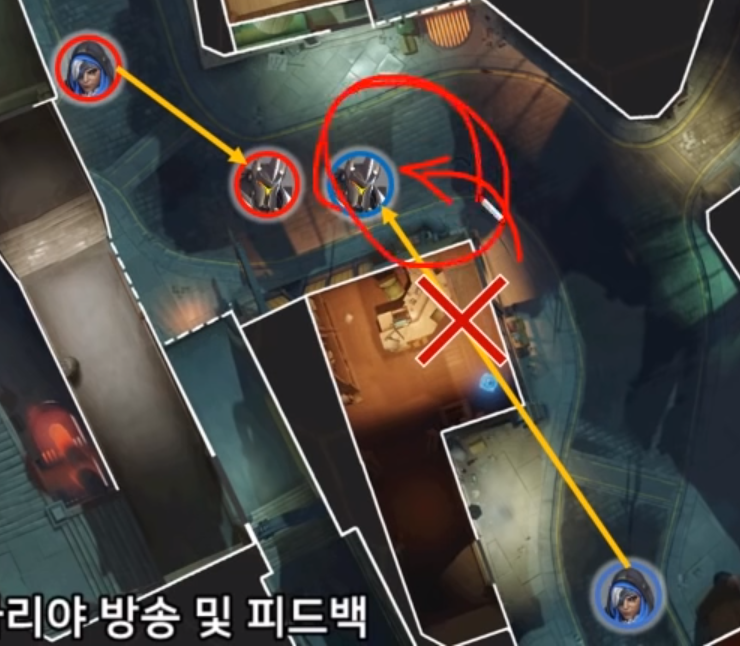
\includegraphics[width=0.6\textwidth]{figures/rz_form/disconneted.png}
    \caption{라자 포메이션 싸움 1: disconnection 발생}
    \label{fig:RZ_1}
\end{figure}
오버워치의 홀딩 위치는 좁은 길목 또는 코너이다. 이를 달리 말하면 진입하는 입장에서 앞라인과 뒷라인의 연결이 끊기는 위치이다.
\begin{figure}[H]
    \centering
    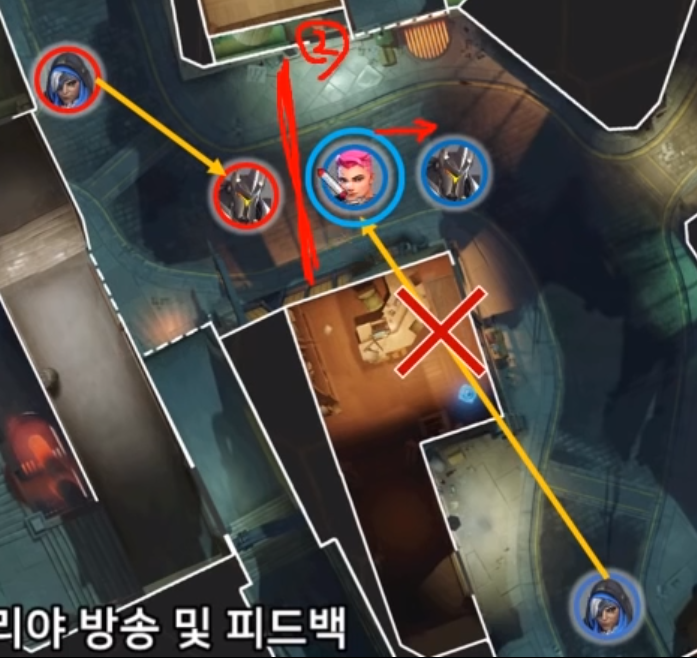
\includegraphics[width=0.6\textwidth]{figures/rz_form/bubble.png}
    \caption{라자 포메이션 싸움 2: disconnection 메꾸기}
    \label{fig:RZ_2}
\end{figure}
따라서 이 잠깐의 힐 공백을 메꾸고 및 진입시 들어오는 압박을 막기 위해 자리야가 라인하르트에게 방벽을 씌워주고, 자가 방벽으로 스스로 엄폐물이 되어 막아준다.

방벽이 모두 소모되기 전에 뒷라인이 연결되어 다시 힐할 수 있는 상태가 되어야 다음 코너까지의 공간을 수비측과 동등하게 사용할 수 있다.
그러나 수비측은 공간을 미리 장악하고 있으므로 이러한 disconnetion이 발생하지 않으며, 같은 방식으로 방벽을 교환할 경우 공격측에 이득이 발생하지 않는다.
따라서 공격측의 플랭킹 경로나 아나의 스킬 변수, 궁극기 교환을 통해 수비를 뚫어낸다.

상대 팀원들 사이의 연결을 윈스턴 방벽, 힐밴, 지형 등으로 막았을 때 변수를 창출할 수 있게 된다.

\section{Attention : 상대의 자원 투자 방향}
상대가 주의력을 어디에 쏟고 있는지도 중요한 판단 기준이 된다.
이 Attention은 State라는 개념으로 팀적으로 구체화된다.

\section{자원의 가치}
\autoref{res:intro}에서 오버워치는 아군의 자원과 상대의 자원을 교환하는 게임이라고 했다. 그런데 자원의 가치는 모두 다르므로, 상대가 가치가 낮은 기술에 자원을 소모하게 하거나 한타에서 제외시켜 자원을 사용할 수 없게 만들거나, 하다못해 자원을 사용하기 까다롭게 만든다면 아군의 사이클을 유리하게 가져갈 수 있다.
자원을 소모시키는 경우와 자원을 사용하지 못하게 하는 경우가 있다. 상대가 초월이 있는 턴에 젠야타를 포커싱해서 잡거나 초월을 먼저 소모하게 한 다음 아군의 자탄 또는 중력붕괴를 써서 한타를 이기고, 젠야타가 늦게 합류해서 초월을 써버린다면 아군의 다음 턴 공격 궁극기를 초월 부담 없이 사용할 수 있게 된다.
이와 같이 상대의 자원을 소모시키거나, 계속 사용하지 못하게 한다면 아군의 사이클을 유리하게 가져갈 수 있다.

\section{마지막으로, Read-Plan-Do-Feedback 루틴에 대하여.}
\begin{enumerate}
    \item 12명 각각의 스킬,궁극기,위치,체력이라는 자원 상황을 사운드와 총알궤적,시야를 통해 파악한다. 이 정보를 바탕으로 12명 각각의 추후 동선과 자원 사용 방향을 읽는다.
    \item  여기서 플레이어 본인의 플레이도 상황에 맞도록-아군은 돕고, 적은 방해하는 방향으로-결정한다.
    \item 계획을 수행한다.
    \item 수행 후 파악하지 못한 정보가 있었는지, 동선과 자원 사용 방향을 잘못 읽었는지, 더 좋은 계획이 있었을지 반추해 본다.
\end{enumerate}

\chapter{Line:오버워치의 전선개념}{\label{sec:state}}
\section{introduction : 오버워치의 상태 구분}
오버워치를 플레이하다보면 푸쉬 콜이나 '빨자' 는 말을 자주 들을 수 있다. 이 장에서는 해당 개념들을 Push, Face-off, Pull이라는 세 State로 체계화한다. 이를 바탕으로 어떻게 State 사이의 전환이 일어나는지 알아보고 각 State에서 자원의 우위를 점하는 방법을 이해한다.
\section{오버워치의 세 가지 상태}
\begin{center}
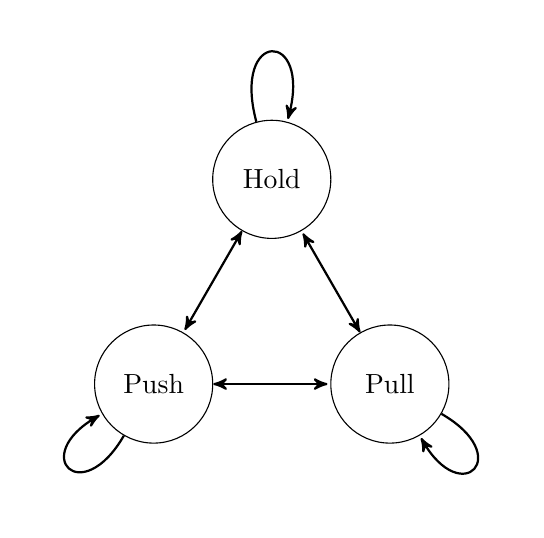
\begin{tikzpicture}[>=stealth', shorten >=1pt, auto,
    node distance=20cm, scale=1, 
    transform shape, align=center, 
    state/.style={circle, draw, minimum size=1.5cm}]
    \node[state] (1) at (1.5,2.6) {Hold};
    \node[state] (2) at (0,0) {Push};
    \node[state] (3) at (3,0) {Pull};
    \path[thick,<->]    (1) edge node{} (2)
                        (2) edge[] node {} (3)
                        (3) edge[] node{} (1);
    \path[thick, ->]    (1) edge[loop above] node{} (1)
                        (2) edge[out=240,in=210, looseness=7] node{} (2)
                        (3) edge[out=330,in=300, looseness=7] node{} (3);
                        
\end{tikzpicture}
\end{center}
\subsection{Hold \& Filter}
상대의 위치 등 정보를 수집하고, 자원 교환을 하는 상태이다. 흔히 오버워치에서 사용하는 오브젝트의 점령 및 화물의 이동을 멈추는 개념보다는 조금 더 넓은 범위로, 유리한 위치에서 상대의 진입을 저지하는 것까지 포함한다. 
홀딩을 하는 조건은 다음과 같다.
\begin{enumerate}
    \item 이 위치에서 홀딩했을 때, 상대의 스킬 투자가 없다면 탱커가 지속적으로 힐을 받을 수 있다.
    \item 이 위치에서 홀딩했을 때, 아군 플랭커들의 스킬을 적게 소모하면서 진입할 수 있고, 원거리 딜링이 유리하다.
    \item 이 위치에서 홀딩했을 때, 상대가 플랭킹하지 않으면(리스크를 감수하지 않으면) 딜각이 좁다.
    \item 상대 대다수가 이 구간을 지나야 한다.
\end{enumerate}
홀딩하는 동안, 다음 변수에 주의한다.
\subsection{Push}
자원을 투자해서 주도권을 가지고 자리를 가져오는 상태
\subsection{Pull}
상대의 자원을 소모시키고 아군의 자원을 모으는 상태
\section{Start State}
\subsection{Hold로부터 시작하는 경우}
궁극기 파밍 및 상대 진형에 대한 정보를 수집한다.
\subsection{Push로부터 시작하는 경우}
자원을 투자해서 주도권을 가지고 자리를 가져오는 상태
\subsection{Pull로부터 시작하는 경우}
상대의 자원을 소모시키고 아군의 자원을 모으는 상태


210715 깨달은 바가 있어서 메모.
Hold도 결국 자원을 투자해야 하므로 Push의 일종이라고 볼 수 있음. 그러나 오직 간보기만.
Push는 메인탱커 뿐만 아니라 본대까지 진입할 수 있는 상황으로 구분.
가운데 단계로 Reset을 추가. 이는 터져서 재정비하는 거라고 생각할 수 있으나 체력관리도 이에 포함됨
Pull 이전에 상대를 흘리는 단계인 Filter를 추가.



\section{State Transition}
\subsection{자원의 우위에 의한 State Transition}
\begin{enumerate}
    \item 스킬 차이
    \item 궁극기 차이
\end{enumerate}
\subsection{진형의 우위에 의한 State Transition} 
\chapter{Line:오버워치의 상태개념}{\label{sec:state}}
\section{introduction : 오버워치의 상태 구분}
오버워치를 플레이하다보면 푸쉬 콜이나 '빨자' 는 말을 자주 들을 수 있다. 이 장에서는 해당 개념들을 Push, Face-off, Pull이라는 세 State로 체계화한다. 이를 바탕으로 어떻게 State 사이의 전환이 일어나는지 알아보고 각 State에서 자원의 우위를 점하는 방법을 이해한다.
\section{오버워치의 세 가지 상태}
\begin{center}
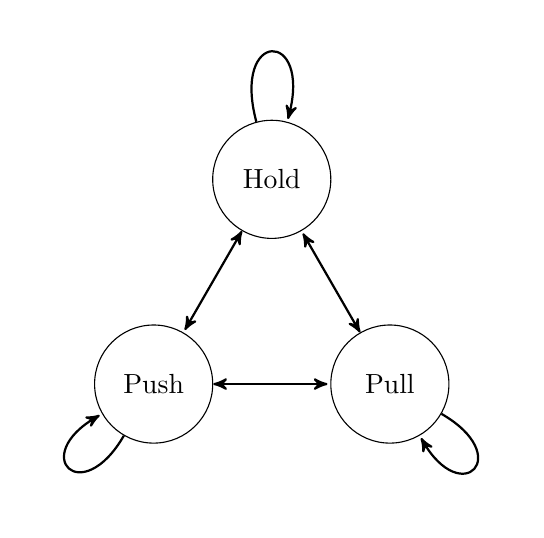
\begin{tikzpicture}[>=stealth', shorten >=1pt, auto,
    node distance=20cm, scale=1, 
    transform shape, align=center, 
    state/.style={circle, draw, minimum size=1.5cm}]
    \node[state] (1) at (1.5,2.6) {Hold};
    \node[state] (2) at (0,0) {Push};
    \node[state] (3) at (3,0) {Pull};
    \path[thick,<->]    (1) edge node{} (2)
                        (2) edge[] node {} (3)
                        (3) edge[] node{} (1);
    \path[thick, ->]    (1) edge[loop above] node{} (1)
                        (2) edge[out=240,in=210, looseness=7] node{} (2)
                        (3) edge[out=330,in=300, looseness=7] node{} (3);
                        
\end{tikzpicture}
\end{center}
\subsection{Hold}
상대의 위치 등 정보를 수집하고, 자원 교환을 하는 상태이다. 흔히 오버워치에서 사용하는 오브젝트의 점령 및 화물의 이동을 멈추는 개념보다는 조금 더 넓은 범위로, 유리한 위치에서 상대의 진입을 저지하는 것까지 포함한다. 
홀딩을 하는 조건은 다음과 같다.
\begin{enumerate}
    \item 이 위치에서 홀딩했을 때, 상대의 스킬 투자가 없다면 탱커가 지속적으로 힐을 받을 수 있다.
    \item 이 위치에서 홀딩했을 때, 아군 플랭커들의 스킬을 적게 소모하면서 진입할 수 있고, 원거리 딜링이 유리하다.
    \item 이 위치에서 홀딩했을 때, 상대가 플랭킹하지 않으면(리스크를 감수하지 않으면) 딜각이 좁다.
    \item 상대 대다수가 이 구간을 지나야 한다.
\end{enumerate}
홀딩하는 동안, 다음 변수에 주의한다.
\subsection{Push}
자원을 투자해서 주도권을 가지고 자리를 가져오는 상태
\subsection{Pull}
상대의 자원을 소모시키고 아군의 자원을 모으는 상태
\section{Start State}
\subsection{Hold로부터 시작하는 경우}
궁극기 파밍 및 상대 진형에 대한 정보를 수집한다.
\subsection{Push로부터 시작하는 경우}
자원을 투자해서 주도권을 가지고 자리를 가져오는 상태
\subsection{Pull로부터 시작하는 경우}
상대의 자원을 소모시키고 아군의 자원을 모으는 상태


210715 깨달은 바가 있어서 메모.
Hold도 결국 자원을 투자해야 하므로 Push의 일종이라고 볼 수 있음. 그러나 오직 간보기만.
Push는 메인탱커 뿐만 아니라 본대까지 진입할 수 있는 상황으로 구분.
가운데 단계로 Charge를 추가. 이는 터져서 재정비하는 거 말고 자원 다시 채우는 단계
Pull 이전에 상대를 흘리는 단계인 Filter를 추가.
Pull 아래 단계로 reset 추가



\section{State Transition}
\subsection{자원의 우위에 의한 State Transition}
\begin{enumerate}
    \item 스킬 차이
    \item 궁극기 차이
\end{enumerate}
\subsection{진형의 우위에 의한 State Transition} 
\chapter{Overflow: 오버워치의 진형과 흐름}{\label{sec:flow}}
\section{introduction : 상황판단}
전선개념 자원체크 당길수있나? 당긴다.


목적:전선 당기기, 유리할때만 싸우기
정보수집, 상황판단-12명 각각의 생각 읽기
간접확인(사운드, 총알궤적), 직접확인 (스킬이펙트, 위치-이동방향 체크) 로 정보 계속 수집
궁극기, 포지션, 스킬 순서로 중요

인간단위 전선확인 포지션 묶음처리 별동대와 본대 구분
시간단위(게임 라운드 포인트 한타 스킬사이클 주의력사이클 딜타이밍-무빙타이밍)  공간단위 코너(주요지형) 인간단위(별동대/본대 개개인) 로 생각
계획-사이클마다할것-해야할것-자원빼기 하지말아야할것(주의해야 할 상대의 변수)
양각제거(간접제거-빠른진입,빠른후퇴,실수캐치, 직접제거-데미지누적 스킬제거, 킬내기 )
양각생성(간접-포인트어그로, 직접-뒷각옆각 반드시엄폐물)
보급로보호
피드백

					    % chapter 2

\chapter{조합별 운영}{\label{sec:comp}}
\section{introduction}
오버워치에 대한 일반론을 많이 설명했지만, 결국 오버워치는 실전을 해야 느는 게임이다. 대표적인 경쟁전 조합(comps)의 운영법을 알아보고, 아군 조합의 운영법과 상대 조합의 대처법을 생각해 본다. 대표적인 조합으로는 33, 오시리둠루모, 러쉬의 계보인 러쉬류 조합, 윈디,윈헴,역병의 사용하는 포커싱 조합,
오호, 레킹볼 3딜, 레디(자)솜파브젠의 원거리 포킹조합 
이 과정에서는 Case를 기억하는 것도 물론 중요하지만, case를 기반으로 일반적인 원칙을 발견하여 기억하는 것을 우선으로 하자. 일반론이 어느정도 체화되었다면, 자원 상황에 따른 detail한 전략적 경우의 수를 계산하고 실행할 수 있어야 한다.
\section{러쉬류 조합}
\input{text/comp/Rush}
\input{text/comp/FullDive}
\subsection{Goats}
\begin{figure}[htp]
    \centering
    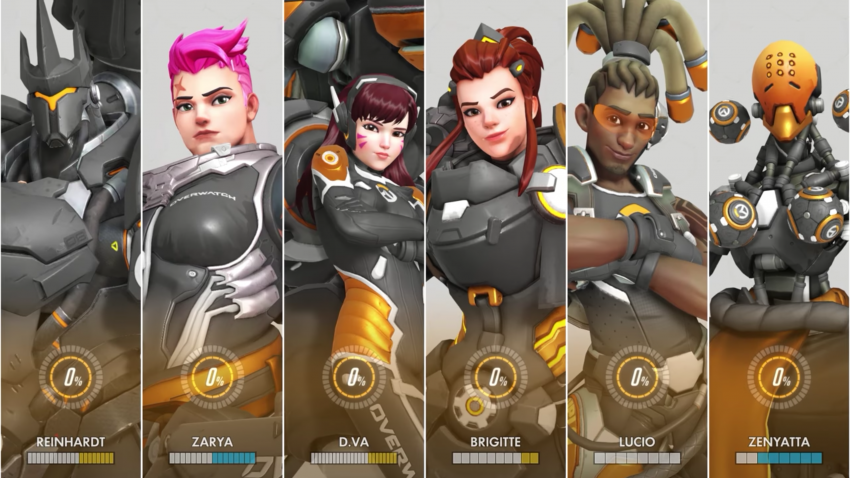
\includegraphics[width=0.8\textwidth]{figures/goats.png}
    \caption{고츠 조합의 기본 영웅들}
    \label{fig:goats}
\end{figure}
\subsubsection{introduction : 브리기테의 출현과 3탱3힐}\label{goats:intro}
오버워치는 4시즌(아나 루시우 젠야타 기용),5시즌(리메이크된 메르시,젠야타) 부터 거의 1년동안 윈디 다이브 조합이 유행하였다. 메르시와 젠야타의 유지력, 탱커들의 기동력과 여기 호응하는 겐지, 트레이서의 포커싱 때문에 원거리 영웅들이 안정적인 플레이를 하기 어려웠다. 이에 블리자드는 2018년 3월, 브리기테라는 새로운 지원가 영웅을 추가해 버티는 조합이 다이브 조합을 이길 수 있도록 만들었다. 당시 50이라는 방밀 데미지로 방밀캔슬을 활용하면 트레이서는 물론 200피 영웅까지 원콤보로 잡을 수 있었던 사기적인 데미지 뿐만 아니라, 600짜리 방패, 방어구를 채워주는 수리킷과 집결이 돌진조합의 핵심 딜량을 깎아버렸다. 게다가 집결을 다 받은 체력 200 영웅은 저격수의 헤드샷에도 죽지 않는 유지력을 보여주었다. 이 뿐만 아니라 방패를 넘어서 기절시키는 방패 밀쳐내기는 서로 라인하르트 대치 조합일 때 망치를 절대 막을 수 없게 만들었다.
이렇게 기존 딜러들 및 탱커들을 브리기테 하나가 전부 카운터해버리자, 아예 딜러를 빼버리고 함께 뭉쳐다니며 빠른 궁사이클과 부조화 포커싱으로 이득을 챙기는 3탱 3힐, 일명 고츠 조합이 등장하게 된다. GOATS!(팀 고츠) 에서는 루시우,모이라, 브리기테를 기용하는 3힐이었지만 여러 조합과의 상성을 고려하여 맞33전을 유리하게 가져가기 위한 루시우, 젠야타, 브리기테를 기용하는 3힐조합이 등장하게 된다.
고츠는 그 어떤 조합보다 케어용 스킬이 많고, 부조화를 이용한 포커싱이 중요하며, 궁사이클이 빠르다. 따라서 팀원들이 가지고 있는 자원을 어떤 순서로 사용할지, 상대의 자원을 어떻게 갉아먹을 수 있을지 팀원들 사이의 원활한 소통을 통해 계획해야 한다. 플레이어 개개인은 본인의 플레이가 팀파이트에 미치는 영향을 제대로 인지하고, 한타에서 본인의 역할을 정확하게 수행해야 한다. ioStux의 goats thesis\cite{ioStux} 를 참고하여 goats 조합의 운영법에 대해 알아보고, 2\-2\-2 조합이 고정된 현 시점에서 적용할 만한 포인트를 짚어보자.
\subsubsection{pre-fight}
궁극기 계산은 모든 한타마다 되어야 한다. 특히 한타 중에 차는 궁극기에 유의한다. 이는 어떤 조합이던지 당연하고, 위에서 설명했기 때문에 자세하게 언급하지는 않겠지만, 굳이 고츠에서 예를 들자면 상대 야타가 초월이 없고 아군 자리야가 자탄이 있다면 아군 자리야는 이 점을 무조건 인지해야한다. \\ 

한타가 시작하기 전에 아군의 자원 사용과 동선을 계획해야 한다. 미리 계획해두면 한타동안 소통의 부재로 일어나는 실수를 줄일 수 있으며, 어떤 궁을 이번 한타에 사용할 것인지 정하고 가야 한타중에 빠른 결정을 내릴 수 있기 때문이다. 한타 전에 계획할 대표적인 요소는 다음과 같다.
\begin{itemize}
    \item 비트 초월이 모두 있다면, 어떤 수비궁을 쓸 것인가?
    \item 어떤 공격궁(탱커궁) 을 사용할 것인가?
    \item 사용하려고 결정한 궁극기를 어느 용도로 사용할 것인가?
    \item 어느 타이밍에 어느 위치에서 그 궁극기를 사용할것인가?
    \item 어디서 홀딩할 것인가? 어디서 (어떤 상황에서) 뒤로 뺄것인가?
\end{itemize}
이를 조합하여 한타를 어떻게 진행할 것인지 계획한다.
\footnote{예를 들어 렐리가 있고, 상대가 막턴을 밟아야하는 상황이라고 해보자. 앞에서 빠르게 치고 들어가면서 앞라인싸움을 유도한다. 상대가 궁이 있고 아군의 카운터궁이 80정도라면 대치하면서 상대 중요 스킬이나 궁이 소모되도록 한다. 등등의 한타의 큰 그림을 그린다.}
 한타 전 계획이 익숙해질수록 지형적 특성과 궁극기 상황에 따라 팀원 개개인이 한타중에 취해야 할 행동을 쉽게 떠올릴 수 있게 된다. 즉, 팀원들간의 소통 없이도 상대의 어떤 약점을 캐치해내야 하는지, 어떤 궁에 대비해야 하는지, 그리고 어떤 궁을 사용해야하는지에 대한 판단이 암기된다. \\
한타 전 계획이 완료되었다면, 다음은 한타유도(initiating) 대해서 알아보자. 이 역시 팀원간 원활한 소통이 중요하다.

한타 중 팀원간 소통에서 주의할 점은 2가지가 있다.

 1. 소통은 언제나 직접적으로; 간접적으로 소통하는것은 고츠에서 최악의 선택임.
고츠의 기본은 속도다. 잘하는 팀은 상대로서 비집고 들어갈 구멍이 작기 때문에 그 작은 구멍을 붙잡고 버텨서 상대 수비를 열어야함. 
그러기 위해서는 팀으로서 확실한 결정을 내려야 할 필요가 있다. 고츠에서는 일단 지르고 그 다음에 생각을 해야한다
예를 들자면, 상대 자리야 자방이 빠졌을때, 저쪽 자방 빠졌으니까 들어갈래? 가 아닌 저쪽 자리야 자방 빠졌다 콜이 들림과 동시에 모든 팀원이 자리야를 포커싱.

 사람들이 하는 가장 큰 착각은 고츠에서 라인이 메인오더를 한다고 생각하는것이다.
하지만 고츠조합은 6명이 하나의 유닛으로서 움직이는게 제일 중요하며 고츠에서 한타 시작은 각각의 플레이어가 아닌 팀원 전체가 하나의 유닛으로 하는 것이다.
쉽게 말해서, 상대가 뇌절하면 누구 한명이 쟤네 누구 뇌절했다, 들어갈래? 가 아니라 팀원 6명 전부 상대가 뇌절했다는것을 인지하고 바로 이득을 봐야함.

Ex) 쟤네 자리야 주방 빠졌다, 라인 포커싱하자! =>ㅇ
     쟤네 자리야 주방 빠졌으니까 라인 노리는거 어때?=>x

 한타의 결과가 좋지 않다면 그것은 당신이 고츠를 이해하지 못하거나 팀원이 고츠를 이해하지 못한 것, 또는 당신의 팀원이 한타을 위한 준비가 안됬던 것이다 ex)포지셔닝,스킬쿨

 한타를 하려고 할때(본인이) 팀원중 누군가가 준비가 안되었다고 하거나 한타유도를하는 것을 거부한다면 그냥 "하지마!" 라고 빠르게 외치고 한타를 그만둬라.
한타를 한다는 콜을 특정 영웅이 하는 것이 아니라, 6명중 누구던지 콜을 할 수 있는것.
단, 6명 모두 한타에 대한 자신의 판단이 확실해야 하며, 판단이 확실하게 서지 않는다면 본인이 이유를 찾아야 한다( 위치선정, 낮은 이해도)

2. 고츠에서 모든 한타는 목표 영웅 하나를 정하고 해야함.
            주방빠졌다! 들어가!=>x
            주방빠졌다! 라인잡아!=ㅇ
명확한 대상없는 포커싱 오더는 팀의 분열을 부른다

 한타를 한다는 것은 상대의 중요한 스킬이나 상대의 위치가 안좋다는것이다. 
따라서 상대는 뒤로 빠지거나 산개하여 피해를 최소화하려고 할것이며,
확실한 목표를 설정하지 않고 한타를 한다면 팀원 6명이 서로 다른 영웅을 목표로 하고 움직이기 때문에 결과가 좋지 않을수밖에 없다.

3.포커싱 대상 호출(taget call)
 한타에 대한 콜을 너무 복잡하게 생각하지 마라.
가장 가까이 있는 영웅을 포커싱 한다는 콜은 아무 문제가 없다.  
허나 안좋은 결과를 만들수 있는 경우가 몇 가지 존재한다.
\begin{itemize}
    \item 상대 앞라인이 건재한 상태에서 그 뒷라인의 영웅을 포커싱 하자는 콜
    \item우리팀 본대에서 거리가 너무 멀리있는 상대팀 영웅에 대한 포커싱 콜
\end{itemize}
데미지 딜링이 신속히 이뤄져야 자리도 쉽게 먹을수 있다.

상대 자리야가 라인옆에붙어있다면 자리야 콜이 맞지만, 거리가 좀 멀다면 우리쪽의 포지션이 무너진다.
자리야에게 이동하다가 라인과 브리기테를 상대해야한다는 것을 보는 순간 자리야 포커싱을 중지하라는 콜을 팀에게 전달하여 멈추는 것이 좋다.
완벽한 타겟을 잡으려고 우리팀의 포지션을 희생하는거 보다 그 타켓을 잡는것을 포기하고 우리의 포지션을 완벽하게 잡는게 더 좋다.

고츠가 특이한점은 누가 콜을해도 이상하지 않다는것이다
돌진조합에서는 윈스턴이 콜을 해야하지만 고츠에서는 라인이 콜하던 자리야가 콜하던 차이가 없음.
글쓴이(ioStux,XL2 코치)의 경우 팀내에서 말이 제일 많고 목소리가 제일 큰사람을 주로 콜 하게 함.
콜을 주로 하는 사람을 팀내에서 정할때는 실험적으로 해도 된다.
특정 영웅을 플레이한다고 메인 콜을 하게 하는 것은 잘못된것.

그러나 콜하는것에 강약조절은 필요하다
목소리가 언제나 크고 말이 언제나 많은 사람이 자잘한 브리핑까지 맡는것은 효율이 떨어짐
정보 전달은 침착하게 해야하며 긴급한 브리핑은 큰소리로 빠르게 해야한다

한타 설계를 실행 할수 있는 것. 그런 강약 조절과 소통이 되어야 완벽하게 한타를 할 수 있다
따라서 자잘한 브리핑을 서로 완벽하게 하는게 중요함. 팀원 모두에게 똑같은 정보가 머리속에 입력되어있는게 제일 이상적.

---명확한 오더 및 한타 중 계획----
마지막으로 소통에 대해 언급하고자 하는 점은 한타 중 계획이다.
한타 전 설계는 매우 중요하지만 한타를 하다보면 계획이 변경될것이다.
서로 고츠조합에 익숙하지 않다면 한타가 오래 지속될것이다.
이럴 경우 한타중에 궁이 예상치 않게 차게 되는 경우가 존재한다(우리팀이든 상대팀이든)

한타전 계획이 미숙하다면 한타중에 차게되는 궁을 연계하기가 어렵다
따라서 브리핑이 활발해야한다
글쓴이의 경우 어떤팀을 잠깐 피드백 했었는데 
그팀은 시도때도 없이 나이스만을 외쳐되서 필요한 브리핑이 전혀 이루어지지 않았다
그런 상황을 방지하기 위해 중요한 내용을 신속하고 침착하게 브리핑 하는것이 중요하다

한타 전 설계를 잘해놓고도 한타 도중에 타겟설정이나 궁 사용에 대한 적절한 소통이 이루어지지 않아
궁을 낭비하거나 포커싱이 흐트러지거나 중요 궁을 너무 아껴 결론적으로 망한다거나 하게 된다
고츠 메타에서 소통은 연속적이여야 하며, 쉬어가는 타임은 없다는 것을 인지해야한다.

고츠조합에서는 한타의 목표가 무조건 상대궁이 빠지도록 유도하는 것은 아니다.
고츠조합에서의 목표는 상대가 뇌절또는 실수하도록 하는 것이기 때문에, 너무 대놓고 궁극기로만 플레이하면 상대가 실수를 하지 않기때문에 목표와 어긋난다
물론 예외는 있다 (6궁 vs 야타 노초월)
또는 추가시간 마지막한타
예를 들면, 왕의길 2거점 화물길은 ㄱ자 길이 많기 때문에 대놓고 자탄자폭콤보로 빠르게 막는것은 오히려 상대방이 한턴 져주고 
리그룹을 빠르게 할 수 있기때문에 효율성을 잘 따져봐야 한다.
한타를 이기고 궁 게이지를 조금 앞서는 것이 한타를 완벽하게 이기고 궁게이지가 바닥나는거 보다 좋다

기본적인 한타유도 3가지
\begin{itemize}
    \item 고지대 한타유도 : 우리팀이 수비중일때 상대방이 고지대를 먹고 내려오려고 할때, 간단하게 가장 먼저 고지대에서 밑으로 내려오는 상대 영웅을 포커싱한다. 예를 들어 리장타워 야시장 맵의 경우, 상대방이 좁은 1층에서 자리싸움을 꺼려하여 2층으로 돌아서온다면, 고츠를 못하는 팀일수록 1층으로 내려오는 속도가 영웅마다 다르다. 주로 라인이 먼저 내려오게됨. 이럴때 라인을 포커싱하여 죽이던가, 상대방의 스킬이 라인을 살리는데 빠지는 상황을 노려 이득을 챙긴다. 또는 상대방이 고지대에 있으면 디바 부스터나 루시우 밀치기로 한명을 떨어트리고 포커싱하는 것도 방법이 된다.
    \item 따로 떨어진 영웅 포커싱 : 상대 디바가 우리 야타를 잡으러 무리한다던지, 상대 브리기테가 본대와 멀어지는 실수를 하는 경우, 따로 떨어진 하나의 영웅을 포커싱하여 잡는다. 이것은 팀원 모두가 언제나 상대 포지션이 떨어져있는지 아닌지를 인지하고 있어야 한다. 앞라인에 주로 있는 라인 자리야 브리기테의 경우 뒤를 잘 못보기 때문에 본대 앞라인 뒤로 들어온 영웅들에 대한 콜을 뒷라인이 적극적으로 해줘야함. 2번의 경우 루시우의 이속 볼륨업이 무조건 필요한건 아니다.
    \item 자리야 주는 방벽 확인 : 상대 자리야 주방이 빠지고 우리는 주방이 있을때 한타를 시작 한다. 별개의 경우도 존재하지만, 90프로 이상의 상황에서는 3번 방법를 한다. 한타유도로 인해 킬이 나면 이상적이지만, 킬이 나지 않았다고 해서 실패인건 아니다. 조심해야 할 것은 한타유도를 한 후 우리팀의 스킬 쿨이 돌고있을때가 제일 위험하고 취약한 상황이다. 그 상황을 다른 스킬 등으로 잘 버티거나 넘기는 것이 좋은 팀이다. 부조화를 이용하는 한타유도도 가능하지만 실패할 리스크가 매우 높다. 자리야 자기방벽이 빠진상태에서 자리야 부조화 같은 경우는 좋은 시도가 될수 있다.
    \item Playing the line이라는 한타유도 방법이 존재 한다. 이는 특정 맵에 가상으로 줄을 그어 놓고 (주로 ㄱ자 길 또는 좁은 길)
대치상황에서 상대방 영웅 중 그 선을 넘은 영웅에게 포커싱을 가하는 하는 것이다.
좋은 예는 하나무라 a거점 수비측. 상대가 정문 조금 앞쪽 라인을 넘으면 6인이 전부 그 영웅을 포커싱.
또한 공격측에서 한명을 따고 거점 한칸을 먹은상태에서 상대가 재정비하고 다시 거점으로 한타하러 올때, 
공격측은 거점 두개의 문에 각각 줄을 그리고 그 선을 넘은 영웅을 어느쪽이든 포커싱.
Playing the line은 상대가 고츠를 잘하는 팀이면 성공률이 떨어진다.


\end{itemize}



레킹볼 3딜 방벽쪼개기 조합에는 2cp맵에서 고츠를 수비에 사용해 궁을 모으고 2거점에서 궁 사이클을 돌리며 막을수 있도록 쓸 수 있다. 단 2거점 입구가 상당히 좁아야 한다
이런경우 1거점에서는 한타유도 보다는 팀원 전원의 생존과 버티기를 위주로 수비한다
한타를 하는 경우는 언제나 상대방이 뇌절했을때
 - 타겟 정하기
한타유도로 첫 킬을 따낸 후 그다음 타겟을 정하는게 매우 중요하다.
첫킬 이후 상대 자리야가 근처에 있다면 자리야를 노리는게 제일 좋다.디바를 노리는 것은 좋지 않다. 고츠조합의 메인 딜 소스를 차단해버린다는 느낌으로 타겟을 잡아라.
특히 자리야는 도주기가 없기 때문에 첫킬 이후 타겟으로 정말 적합하다.

자리야 디바를 보기 어렵다면 라인의 방벽에 타겟을 잡아주자. 한타가 껄끄러워 질때쯤 상대 라인의 방벽이 관리가 안되게 된다--> 아군 대지분쇄로 한타 정리 가능.
도주기가 있는 대상은 타겟으로 왠만하면 잡지 않는것이 좋다. 갑자기 타겟이 없어져 팀의 한타에 비는시간을 만들기 때문
루시우를 한번에 죽일거 아니면 그 딜을 상대 라인 방벽에 꼬라박는게 더 낫다.



---기술---
-조화의 구슬
HPS(초당 힐량)는 단순히 HPS가 아니다. 체력을 3가지 단위로 구분하면 아머> 체력> 쉴드인데, 
따라서 이상적으로는 조화의 구슬을 아머가 존재하는 영웅에 달면 숫자로는 60의 데미지를 막을수 있는것.
이상적으로는 아머가 있는 영웅에게 조화의 구슬을 달면 2배의 효율을 낼 수 있지만, 실제로는 그렇지 않다. 하지만 효율이 더 올라가는것은 맞다.
아머가 이미 남아있는 영웅보다 아머가 없는 영웅이 더 체력적으로 약한것==> 따라서 조화의 구슬이 자리야에 달려있다면 
그것은 다른 관점으로 본다면 상대방이 아군의 라인하르트의 아머를 깎을수 있는 기회가 되는것
이는 아군 라인의 체력저하로 이어지며 아군 라인이 부담이 되 자리싸움에서 밀리거나 심각한상황에서는 죽게되는 상황까지 이를 수있게됨.
또는 수비형 스킬들이 빠지는 결과를 초래하게됨(자리야 주는방벽)
따라서 조화의 타겟팅은 한타 시작전에는 라인에 있는게 제일 이상적임.
또한 수준높은 라인하르트는 자신에게 조화가 고정되어있다는 생각을 하고 플레이를 할때가 많음.
다른 두 탱커영웅들은 브리의 힐량이나 루시우의 힐량정도로 생존이 가능하기때문에 조화는 왠만하면 라인에게 고정하는것이 정답,
또한 조화는 힐이 급할때 쓰기 보다는 지속적으로 달아놓는게 더 효율이 좋다. 예를 들어, 우리 자리야가 포커싱당하는데 거기다가 조화를 달아준다고 결과가 크게 달라지지는 않는다.
요점은 라인의 아머가 최대한 오래동안 남아있도록 조화를 고정해주는것. 고츠에서 위급한 상황에서의 힐은 브리의 수리팩이나 자리야의 주는방벽임.

-부조화의 구슬
부조화 메인 타겟팅은 상대 라인하르트가 되어야함. 야타 본인이 떄리는 대상이 라인이 아니더라도 가능하면 부조화는 라인에게 고정.
또한 부조화를 라인에 달음으로서 상대 자리야 주는방벽이 라인쪽으로 빠지도록 유도 후 다른 영웅을 포커싱하는 전법도 사용할 수 있게 된다.
상대 라인에게 부조화가 달리는 것 만으로도 엄청난 부담이됨.

-자리야 방벽
자리야 방벽을 잘못쓰는 것이 고츠 미러전에서 지는 가장 크고 잦은 이유이다.
자리야가 아군라인에게 방벽 원하는 타이밍 콜해달라는 것은 좋지 않음. 절대 하지 말것.
주는방벽 타이밍은 자리야 플레이어의 책임이 동반되어야한다.
라인에게 주방 콜 해달라는건 정말 하지말라고 강조하고있음.
자리야 본인이 알아서 타이밍 재서 쓰는게 가장 효율적.

중요한 것은 스킬을 마지막 순간까지 아끼는것.
가장 좋은 예는 자리야 방벽과 젠야타 초월.
늦게 쓸스록 이득을 많이 볼 수 있음.
허나 늦게 쓴다는건 팀원과의 믿음이 견고해야함.
타이밍 안맞으면 팀웍이 떨어지게됨.
스킬을 아끼는 것이 중요한 이유는 자리야 방벽의 경우 일종의 치킨게임이기떄문.
얼마나 이 치킨게임에서 우위를 점하느냐에 따라 상대 자리야에 우위를 점할 수 있음.
또한, 자리야 방벽을 이렇게 쓸 경우 브리기테 수리팩으로도 많은 이득을 볼 수 있음.
풀피 라인에 주방주는거는 딱 두가지경우에만 하도록 
1. 라인이 방벽이 다 꺠졌고 라인앞에 자폭이 있을떄 
2. 라인이 상대 라인에 돌진맞아 제압되어있을떄

그외에는 먼저 주방을 쓰는건 상대에게 한타를 시작할 타이밍을 주는 행위.
고츠에서는 사실 주는 방벽을 안써도 되게 상황을 만드는것이 정말 좋음.
거두절미하고 아군 라인이 상대쪽으로 풀피상태로 뛰어드는데 주방을 줬다면 그건 자리야가 게임을 던진거다. 주방은 긴급탈출버튼이다.
주방에 대한 상황은 4가지
1. 우리가 먼저쓰고 상대가 안씀. 
2. 저쪽이 먼저쓰고 우리가 안씀. 
3. 저쪽이 먼저쓰고 우리가 몇초 있다 쓴다. 
4. 우리가 먼저쓰고 저쪽이 몇초 있다 쓴다.

1상황: 절대 하면 안된다. 이런 상황이 벌어지는건 보통 조화가 라인에 고정이 안되있다거나 라인이 방벽을 제떄 안들어서 부조화맞고 압박당한다거나.
이런 상황이 벌어진다면 1순위 목표는 생존.
상대 자리야가 아군 주방이후 무조건 주방을 쓴다는 확신이 있으면 먼저 주방을 써라.

2상황: 이 경우 생각해볼수 있는 것은 다음 주방이 돌아올때 상대방 주방이 쿨타임이라는 것.
이런경우 보통 콜이: 저쪽 주방 썼고 우리 주방 곧 온다.. 3..2..1...
이 콜을 듣고 아군 모두는 본대가 한타를 유도하러 들어갈 것이라는 것을 인지해야한다.

3상황: 이것이 가장 좋은 방법이라고 할수 있다.
만약 이상황이 발생하면 적군팀의 오더나 브리핑을 꼬거나 힘싸움에 있어 많은것을 우리에게 유리하게 되도록 상요할수 있다.
자리야 방벽이 사라지자 마자 진입을 하면 된다 2~3초의 자리야 방벽으로 인한 이득보다 우리팀에게 싸움에서 이기기 충분한 8초의 시간을 줄수있다
그러나 이 상황이 발생하였을때 이기지 못한다면 이점이 사라지고 불이익이 발생할구 있다 상대는 우리의 실수를 유도 하기 위해 노력할 것이다
이 상황을 이용해 가장 큰 이득을 보려면 본인(자리야)의 자신감이 확실하고 젠야타의 구슬 고정을 확인하며, 상대 포커싱에 대한 오더가 일관되고 빠르게 진행되야 할것이다

4상황:가장 나쁘지는 않지만 좋지도 않다. 물론 먼저 주방을 사용하기 위해 적의팀을 시험하고 죽여야 하지만 다시 한타를 여는것에 대하여 신중해야 한다
우리팀이 아무도 죽이지 않고 목표(거점,화물)을 점거하고 있고 그들이 무엇을 하고 있는지를 안다면 주방 쿨타임이 돌기전에 상대팀이 우리를 죽이려 할것이다
우리가 주방을 먼저 주었을때 무언가를 죽일수 있다고 생각하지 않는다면 뒤로 빠져 다시 한타를 열어 중립적인 상황에서 다시 돌아온 주방 쿨타임을 이용해서 
한타를 열어야 할 것이다

이 4가지 상황을 모두 이해하는것이 중요하다,
팀원 모두가 이 4가지 상황 모두에서 할 일을 이해해야한다
누군가가 이 상황들을 식별하는데 어려움을 겪는다면
자리야가 방벽을 사용할때 오더와 브리핑에 있어 더 많은 점유율을 차지 하는것이 
도움이 될수 있다.

자리야가 일방적으로 이득을 취하는 방법은 적에게 과도한 궁사용을 유도해 다음 싸움을 압도하는 것이다.
이를 위해 방벽 훼이크(원문은 bating bubbles이나 이렇게 함)가 유용하다 이것은 적팀이 2상황에 들어가게 하는 것을 미끼로 하는 방법이다.
이것은 매우 간단하다 가짜 교전을 하고 아군 라인이 풀피일때 방벽을 사용하고 상대라인에게 압박을 넣는척 해라
이것은 상대를 죽이거나 공간을 차지할 목적으로 하는것이 아닌 상대가 우리팀이 뇌절한것 처럼 보이게 하여 궁극기를 사용하게 하는것이다.
이 과정에서 궁극기를 빼지 못하더라도 상대 주방의 쿨타임을 계산하여 4상황을 유도해 한타를 비등하게 가져갈수도 있다.

자리야에 대한 마지막으로 자탄 자폭에 대해 설명하고 이것이 방벽에 어떻게 영향을 미치는지 알아야한다
적이 자탄자폭을 가지고 있다면 초월은 일반적인 상황에서 의미가 없다
방벽이 라인을 방밀한다면 팀은 초월이나 비트를 써도 일반적으로 죽게 될것이다.
상대가 자탄 자폭 콤보 각을 보고있다는 것을 안다면 자리야는 방벽관리, 특히 자기 방벽관리에 대해 주의할 필요가 있다.
많은 자리야가 싸움전에 에너지를 위해 자방을 사용하는 것을 선호하지만
적팀이 자탄자폭을 가지고 있고 자방을 이미 사용했다면 그 콤보로부터 자신이든 팀이든 보호할수 없을것이다,
자리야의 자방은 자탄자폭으로부터 팀을 구할수 있는 훌륭한 기술이다.
왜냐하면 그것은 자폭의 중심점으로부터 나오는 폭발을 완벽히 차단할수 있기 떄문이다.
Uprising Acadamy(보스턴 아카데미 팀) 에서 lced선수는 자탄자폭으로부터 팀을 구하는 자기방벽 사용법을 완벽히 연습한후 그것을 해냈다.

디바 매트릭스 사용법
다음으로 방어 매트릭스에 대해 이야기 해보자
그것은 매우 간단하다 
매트릭스를 한타 초반에 사용하여 충전하는것은 더 많은 피해를 막을수 있게 한다
따라서 라인하르트의 방벽과 체력을 더 많이 보존시키며 상대 젠야타의 궁 게이지를 늦추고 시작하는 효과적 방법이다
자리야 자탄을 먹을때도 충전된 매트릭스를 계속 키는것으로 쉽게 먹을수 있다.

적 자리야가 자탄이 없다면 매트릭스를 라인하르트가 방패를 들지 않고 한타참여를 위해 망치를 휘두를떄 사용할수 있다
매트릭스를 키는동안 상대 자리야는 자탄을 사용하지 못하므로 좋은 자탄각을 볼수 없게 될것이다 
모든 자탄을 먹을수는 없지만 자리야를 특정 포지션 그리고 특정 타이밍에 자탄을 쓰게 하는 것만으로도
이는 큰 가치가 있다.

아나를 사용한 고츠를 쉽게 카운터 치기 위해서는 아나위주로 매트릭스를 사용해야 할것이다:D
아나의 힐벤과 힐을막아 아나의 기여도를 크게 떨어뜨려 젠야타를 기용한 우리팀이 압도할수 있도록 할수 있다
이는 또한 우리팀이 아나의 힐벤이 의미가 없다는것을 알기때문에 상대가 젠야타를 기용한것보다도 더욱 쉽게 진입할수 있는 기회를 준다
그러나 이를 하지 못한다면 힐벤으로 인해 팀이 터져나갈것이다.

-라인하르트 스킬 사용
물론 라인하르트의 스킬 사용은 상황에따라 거의 무한한 가짓수의 사용법이 나올수 있다
하지만 우리가 절대로 지켜야할 사용방법이 하나가 있다 
이것은 자탄자폭에서 자폭방향으로 방패를 무조건 드는 것이다:D
자탄 자폭 콤보가 상대방에서 나올때까지 방벽을 유지하는것으로 아군 자리야에게 안정감을 줄수있다
자탄 자폭이 상대방에게 없는것을 아는 상황에서는 방패를 아끼지 말고 들고 팀과 함께 빠르게 자리를 먹는것이 좋다

아군이 자탄자폭을 사용할때 돌진을 사용하는것은 매우 중요하다 
너무 일찍 돌진을 사용한다면 상대 라인하르트가 대지분쇄로 아군을 눕히고 자폭을 방어하기에 충분한 시간을 줄것이다
따라서 자폭이 거의 다 터져가는 마지막 순간에 짧은 거리에서 돌진을 사용해야한다.
그러나 무엇보다도 생존이 중요하다
만약 이 돌진으로 인해 자신이 죽는다면 아군은 이미 자탄 자폭을 사용했기 때문에 리그룹을 하는 상황에서 손해를 볼수 있고
자탄 자폭 콤보가 실패 했을시에는 상대가 아주 쉽게 싸움을 가져갈수 있기 떄문이다.

잘하는 디바들은 화염강타를 대부분 먹을 것이지만 
그것의 목적과 가치를 이해하는것은 중요하다
화염강타는 적을 약화시키고 압력을 가하고 공간을 차지하는 방법이다
5명에게 화염강타를 적중시킨다면 그것을 치료하는데에 적은 많은 시간이 필요할것이고
필연적으로 우리팀은 더 많은 더 좋은 공간을 차지할 수 있다
네팔 신전을 예를 들자면 계단을 올라가는순간 화염강타를 던졌을때 6명을 적중시킬수 있다
우리팀은 그로 인해 압력을 더 크게 가할수 있고
상대는 부족한 체력으로 인해 거점에서 싸움을 유도할수 없을것이다
디바가 처음 화염강타를 먹지 않을거 같지는 않지만
이런효과를 이용하기 위해 첫 화염강타는 매우 중요하다.

화염강타는 다시 한타를 여는것에도 매우 좋다
그것은 망치질 한번보다도 데미지가 높기 떄문에 아머류 체력을 깎는것에 효과적이고
관통효과도 있기 때문에 체력이 낮은 적 젠야타를 킬할수도 있다.
그리고 적 디바에게 매트릭스를 사용하는 것을 강요해서 아군 자리야에게 더 쉽고 좋은 자탄각을 열게 할수도 있다.

화염강타를 최고의 방법으로 사용하게 하려고 하는것은 매우 중요하다
고츠를 잘 사용하는, 약간 차원이 다르다고도 느껴지는 팀들을 잘 관찰하면 화염강타 사용법이 매우 중요하다는 것을 느낄수 있을것이다.

-브리기테
---방밀 사용법---
이는 3가지로 나눌수 있다
1.이동기
2.킬결정
3.젠야타와의 연계(5orbs setup이라 되있는데 이는 추후 설명)

일단 기동성으로 사용하는 방법은 주로 합류할떄 사용하거나 적을 추격하게 사용하게 될것이다 
이는 꽤나 자주 사용하고 누구나 할수 있기 떄문에 긴 서술은 하지 않는다.

그리고 킬결정으로 사용하는것은 매우 중요하다
팀이 라인하르트에게 압력을 가하기 시작할때 상대 라인하르트는 망치질을 하다가 아머가 까이는 순간 방패를 들것이다
이 찰나의 틈에 상대 라인에게 방밀을 한다면 라인을 죽여 한타를 가져가거나 상대의 자리야 방벽을 유도할수 있다
방밀의 스턴시간은 1초로 부조화와 함께라면 상대 라인하르트의 체력 300정도는 상대의 케어를 거의 무시하고도 없앨수 있을것이다
물론 상대도 이 사실을 알기때문에 맞돌진을 시도할것이다
맞돌진을 당한다면 자리야 방벽싸움에서 밀리거나 브리기테가 죽기때문에 썩 좋은 결과는 보지 못할 것이다

젠야타와의 연계(5orbs setup)는
일종의 공격형 궁극기와도 비슷한 효과를 낼수 있다
이는 엄청나게 효과적이며 궁극기를 사용하지 않고도 한타를 이길수 있을것이다
그러나 이를 시행하는것은 아군과의 합이 완벽하다고 말할수 있을정도로 잘 맞춰져야 할것이다

젠야타와의 연계는 매우 간단하다
젠야타가 구슬 5개를 모으면 브리기테는 방밀에 대한 카운트 다운을 한다
방밀과 함께 젠야타가 구슬 5개를 발사한다면 적군은 400에 달하는 데미지를 입고 곧 죽게 될것이다.
사실 이는 몇번 일어나지 않는 상황이며 글쓴이도 한번밖에 본적이 없다...

이를 완벽하게 사용할수 있는 팀이 있다면 글쓴이(coaching@iostux.com)에게 메일이나 트위터 DM을 보내주길 바란다.
글쓴이는 그 팀의 스크림을 관전하기 위해 큰 돈을 지불할 것이다:D

---수리팩 사용법---
브리기테의 수리팩은 자리야의 방벽과 매우 흡사하다
150힐량으로 슈퍼 세이브를 할수도 있고
75의 방어구로 팀에게 안정감을 부여할수도 있다
이것을 당신이 올바르게 사용한다면 아마 대부분 아군 라인하르트에게 사용하는 때일 것이다
이상적인 경우는 자리야 방벽이 라인하르트에게 들어가기 전에 사용해야하며
그렇기 때문에 라인하르트는 팀을 신뢰하는것이 중요하다
이 타이밍이 잘 맞지 않으면 그는 300hp에서 폭발적인 힐을 받지 못해 죽거나 너덜너덜한 상태가 되며 자리야 방벽이 쉽게 빠질것이다

이상적인 타이밍은 라인하르트가 300~350체력이 되었을때 브리기테의 수리팩을 풀피 상태로 만든다
그리고 다시 체력이 내려갈때 자리야가 그에게 방벽을 씌우고 조화,브리기테 패시브,루시우의 힐이 그를 다시 풀피로 만들것이다
적어도 그에게 수리팩을 잘 준다면 힘싸움에서 크게 밀리지는 않을것이다
하지만 이는 이상적인 이야기이고
무언가 죽고 있다면 최우선적으로 그것에게 주어야 한다


-방어구 관리
마지막으로 라인하르트의 아머 관리에 대해 알아보자
명확히 하기 위해 예시를 들어보자
고츠 조합에서 압박을 넣는 단계에서(적팀이 방벽을 사용하게 하려고 하는경우)
우리가 압력을 가하고 있다면 망치를 계속 휘두르다가 아머가 사라졌을때 방패를 들면 된다
이보다 일찍 방패를 든다면 적 자리야가 방벽을 사용하지 않고 우리팀이 에너지를 수급할수 없으며
충분한 압력을 가하지 못할수 있다

아머를 잃지 않고 가능한 한 많은 망치질을 하는것은 압력의 양을 극대화 하는 방법이다
팀은 스킬을 사용하고 싶지 않을것이다.
왜냐하면 아직 완전한 한타를 벌일 이유가 없기 때문이다
따라서 망치질을 할때 브리기테 패시브,조화,루시우 힐에게만 의존하게 될것이다

망치질을 할때 적 자리야가 자방을 사용하지 않는다는 것을 파악했을때 체력과 아머를 올바르게 관리하는지 알아야한다
자방이 안빠진다는것은 자신이 너무 방패를 빨리들고 우리팀이 최대한의 치유를 활용하지 못한다는 것이다

고츠 미러전에서 두팀이 다 잘하는 팀일때 절대로 방패가 먼저 깨지면 안된다
이렇게 된다면 이후 싸움에서 충분한 압력을 가할수 없기 때문이다



\section{갉아먹기 나노파밍 조합}
\subsection{브리기테와 함께하는 다이브 조합}
\subsubsection{introduction : 브리기테의 사기성}
오버워치 전성기의 패왕이었던 윈디 조합은 222 고정과 2방벽 이후 벨런싱이 어느 정도 마무리된 현재 사용되지 못하고 있다. 이 이유는 윈스턴 또는 디바의 다이브를 처음부터 차단할 수 있는 브리기테의 도리께 투척 때문이다\footnote{부가적인 이유로는 윈스턴의 방벽 및 디바의 매트릭스와 상관없이 힐이 가능한 수리킷}\footnote{그래서 브리가 못하거나 안 나오면 디바를 쓰는 게 더 좋다고 생각함.}. 디바를 기용할 경우 윈스턴의 방벽과 상대 브리기테의 shift를 교환해야 하므로 너무 큰 낭비가 생긴다. 따라서 이를 막기 위해 자리야를 사용하게 되었다. 주는방벽과 동시에 다이브할 경우 브리기테의 밀쳐내기를 막을 수 있을 뿐만 아니라 방벽 사용 전 데미지를 흡수할 수 있기 때문이다.

\subsection{기본 조합 : 윈자애트아브}
힐러 및 자리야로 구성된 본대, 윈스턴과 트레이서로 구성된 별동대, 애쉬의 말뚝딜의 삼박자로 구성된 갉아먹기 조합이다. 상대의 진입을 차단하면서 궁극기를 모은 뒤, 자원의 우위가 확실할 때 자리를 먹게 된다.  
\subsubsection{윈스턴의 역할}
\subsubsection{자리야의 역할}
\subsubsection{애쉬의 역할}
\subsubsection{트레이서의 역할}
\subsubsection{아나의 역할}
\subsubsection{브리기테의 역할}
\section{포킹 조합}
\input{text/comp/ballsig}
    % \begin{figure}
    %     \centering
    %     \includegraphics[scale = 0.2]{figures/step5.png}
    %     \caption{STEP 1 ~ STEP 5를 수행한 후 μvision 화면}
    %     \label{fig:step5}
    % \end{figure}
% \clearpage

                       % chapter 3

% \section{토의}{\label{sec:disc}}



% \clearpage

					% eval

 			% related

% \input{text/6_reference.tex}			% conclusion

% \input{text/Appendices.tex} 					% additional chapters

%%%%%%%%%%%%%%%%%%%%%%
% References Section %
%%%%%%%%%%%%%%%%%%%%%%

% \addcontentsline{toc}{section}{참고 문헌}		% Add references section to table of contents
\printbibliography[title={참고 문헌}]
\clearpage

% \input{text/abstract_english.tex} 			    % Text for acknowledgement

% \input{text/acknowledgement.tex} 			    % Text for acknowledgement


% \bibliography{ref}				                % Add bibliography file
% \bibliographystyle{ieeetr}			    	    % Set bibliography style


\end{document}
